\documentclass{beamer}
\usepackage{graphicx}

\usepackage{algorithmicx}
\usepackage{algorithm2e}

\usepackage{pgf} %permet d'introduire des images vectorielles pour les présentations 
\usepackage{tikz} %permet de créer des graphiques dans le texte 


\usetheme{CambridgeUS}

\title{TEST 2 Beamer}
\author{Derrez Lorenzo}
\date{llllll}

\begin{document}

\begin{frame}
    \maketitle
    \centering % centre toute la suite de la frame 
    \begin{block}{Titre du block 1}
        \begin{itemize}
            \item Mon premier point : 
        \end{itemize}
    \end{block}
\end{frame}

\begin{frame}
    \begin{center} % Permet de centrer tout ce qu'il y a dans la commande au lieu de centrer tout ce qu'il y a dans le reste de la frame
        \begin{block}{b2}
            ceci est le block 2.
        \end{block}
        \begin{block}{block 3}
            ceci est le block 3.
        \end{block}
    \end{center}
\end{frame}

\begin{frame}
    
    %a mettre absolument pour commencer un environnement TikZ
    % dans cet environnement, chaque instruction doit se terminer par ' ; ' !
    %si le graphique ne comporte qu'une unique instruction il suffit de faire \tikz
    \tikz \draw(0,0) -- (1,2);

    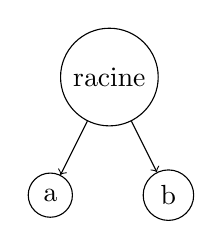
\begin{tikzpicture}[nodes={draw, circle}, ->]
        \node{racine}
            child{ node{a}}
            child{ node{b}};
    \end{tikzpicture}

\end{frame}

\end{document}